\subsection{Funktionsweise der Optischen Wellenleitern}
\label{subsec:poffunktionsweise}

Informationen werden mittels Intensitätsmodulationen der Lichtstrahlen
übertragen. Dabei wird das Licht durch einen transparente Kern, welcher von
einem Mantel umgeben ist, gesendet (siehe \autoref{fig:pofprinzip}). Die
Brechzahl $n$ des Kernes ist dabei größer als die des Mantels. Dies ermöglicht
eine Totalreflexion\footnote{Beinahe vollständige Reflexion von Licht an der
Grenzfläche zweier Materialien} des Lichts am Übergang von Kern zum Mantel.
Aufgrund der Laufzeitunterschiede zwischen den beiden Strahlen in
\autoref{fig:poflichtausbreitung} wird die Bandbreite beschränkt. Die Bitraten
erhöhen sich bei kürzeren Strecken, da sich die Unterschiede zwischen den
Laufzeiten verringern. Durch die Totalreflektion kann das Licht auch durch
Biegungen geleitet werden.

\begin{figure}[h]
    \begin{center}
        \begin{minipage}[t]{0.4\textwidth}
            \begin{center}
                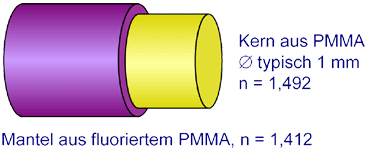
\includegraphics[width=0.9\textwidth]{Bilder/Optische_Wellenleiter_Die_Polymer_Optische_Faser/Funktionsweise/pofprinzip.png}
                \caption[Aufbau eines Kabels aus POF \newline \url{http://www.pofac.fh-nuernberg.de/pofac/de/was_sind_pof/images/pof_prinzip.png} (zuletzt aufgerufen am 19.09.2015)]{Aufbau eines Kabels aus POF}
                \label{fig:pofprinzip}
            \end{center}
        \end{minipage}
        \hspace{0.025\textwidth}
        \begin{minipage}[t]{0.4\textwidth}
            \begin{center}
                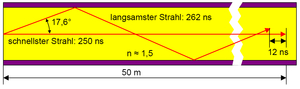
\includegraphics[width=0.9\textwidth]{Bilder/Optische_Wellenleiter_Die_Polymer_Optische_Faser/Funktionsweise/poflichtausbreitung.png}
                \caption[Ausbreitung von Licht in einem optischen Wellenleiter aus PMMA \newline \url{http://www.pofac.info/typo3temp/pics/7eee584dce.jpg} (zuletzt aufgerufen am 19.09.2015)]{Ausbreitung von Licht in einem optischen Wellenleiter aus PMMA}
                \label{fig:poflichtausbreitung}
            \end{center}
        \end{minipage}
    \end{center}
\end{figure}
